\documentclass[10pt, reqno, letterpaper, twoside]{amsart}
\usepackage[margin=1in]{geometry}

\usepackage{amssymb, bm, mathtools}
\usepackage[usenames,dvipsnames,svgnames,table]{xcolor}
\usepackage[pdftex, xetex]{graphicx}
\usepackage{enumerate, setspace}
\usepackage{float, colortbl, tabularx, longtable, multirow, subcaption, environ, wrapfig, textcomp, booktabs}
\usepackage{pgf, tikz, framed, url, hyperref}
\usepackage[normalem]{ulem}
\usetikzlibrary{arrows,positioning,automata,shadows,fit,shapes}
\usepackage[english]{babel}
\usepackage{hyperref}

\usepackage{microtype}
\microtypecontext{spacing=nonfrench}

\usepackage{times}
\title{Indoor-Outdoor Localization for Ground Robots using Factor Graphs}
\author{
Evan Grant [edgrant@seas],
Rithwik Udayagiri [rithwiku@seas],
Aadith Kumar [aadith@seas],
}

\begin{document}

% \input{instructions}

\begin{abstract}

This project implements algorithms for localization in environments comprising both indoor and outdoor regions on the AgileX Scout 2.0 ground robot outfitted with a Velodyne VLP-16 LiDAR and GPS. Our work presents a factor graph-based approach to localization. We perform sensor fusion between LiDAR and GPS data using the GTSAM library \cite{Dellaert_gtsam2012} in hybrid maps where LiDAR alone may be insufficient. A highly accurate map was collected using the 3D Graph SLAM approach from \cite{hdl2019} and LiDAR localization in subsequent trials was performed using the same library. A set of waypoints were manually placed in the map and autonomously tracked using Pure Pursuit \cite{pure_pursuit_1992} to complete a loop through Penn Engineering buildings. We confirmed that LiDAR localization predictably failed in the outdoor region of our map. As the outdoor region of our test environment is surrounded by tall buildings, we were unable to obtain GPS data consistently. Thus we evaluated our sensor fusion algorithm using a simulated dataset derived from actual map waypoints and synthetic noise. The filtering result from the factor graph produced excellent tracking in both indoor and outdoor regions of the simulated trajectory - following the LiDAR estimate closely in indoor regions and appropriately incorporating GPS and odometry readings in outdoor regions where LiDAR lost localization entirely.

\end{abstract}

\maketitle

\section{Introduction}

Localization plays a crucial role in enabling robots to navigate safely around obstacles and follow pre-planned trajectories. However, the techniques currently used in the industry are typically optimized for either indoor or outdoor settings. Consequently, algorithms and sensors designed for indoor localization often do not perform well in outdoor environments and vice versa. To overcome this challenge, we are exploring the fusion of multiple sensor modalities and localization outputs to achieve robust positioning results for both indoor and outdoor spaces.

Indoor-outdoor localization has numerous practical use cases, such as robots that can navigate through a building and then move outside to a parking lot to complete a task, or robots that can traverse a warehouse and then navigate outside to a loading dock for a job. By addressing this challenge we can help enhance the versatility of robots and broaden their scope of applications.

Factor graphs are a powerful tool for solving complex probabilistic inference problems because they can represent the underlying conditional dependencies between variables in a compact and efficient way. Accordingly, their use is becoming common for localization and mapping applications.

For this project, we employed HDL Graph SLAM to carry out mapping and localization tasks. To follow pre-planned trajectories, we used a Pure Pursuit controller. Additionally, we developed a factor graph based sensor fusion algorithm to combine GPS, odometry, and LiDAR data.

To test the performance of an existing algorithm, we employed a purely LiDAR based localization approach with Pure Pursuit on an AgileX Scout 2.0 robot. We also evaluated the effectiveness of our sensor fusion algorithm using a simulated dataset derived from actual map waypoints and synthetic noise.


\subsection{Contributions}

\begin{itemize}
    \item Developed a sensor fusion algorithm using factor graphs via GTSAM to fuse GPS, odometry and LiDAR data to perform seamless indoor-outdoor localization.
    \item Used graph-based SLAM algorithm to perform mapping and localization on real hardware
    \item Developed a pure pursuit controller algorithm to follow a trajectory
    \item Completed extensive setup of hardware, sensors, ROS and Jetson to demonstrate on the real robot.

\end{itemize}

% \section{Related Work}

% Note down references. Say how they relate to your approach. Your objective to put your work in context of the broader literature, namely, what other possible approaches exist for this problem, what they are good at or what they lack, what your approach does differently from them

\section{Approach}
\begin{wrapfigure}{R}{0.4\textwidth}
  \begin{center}
    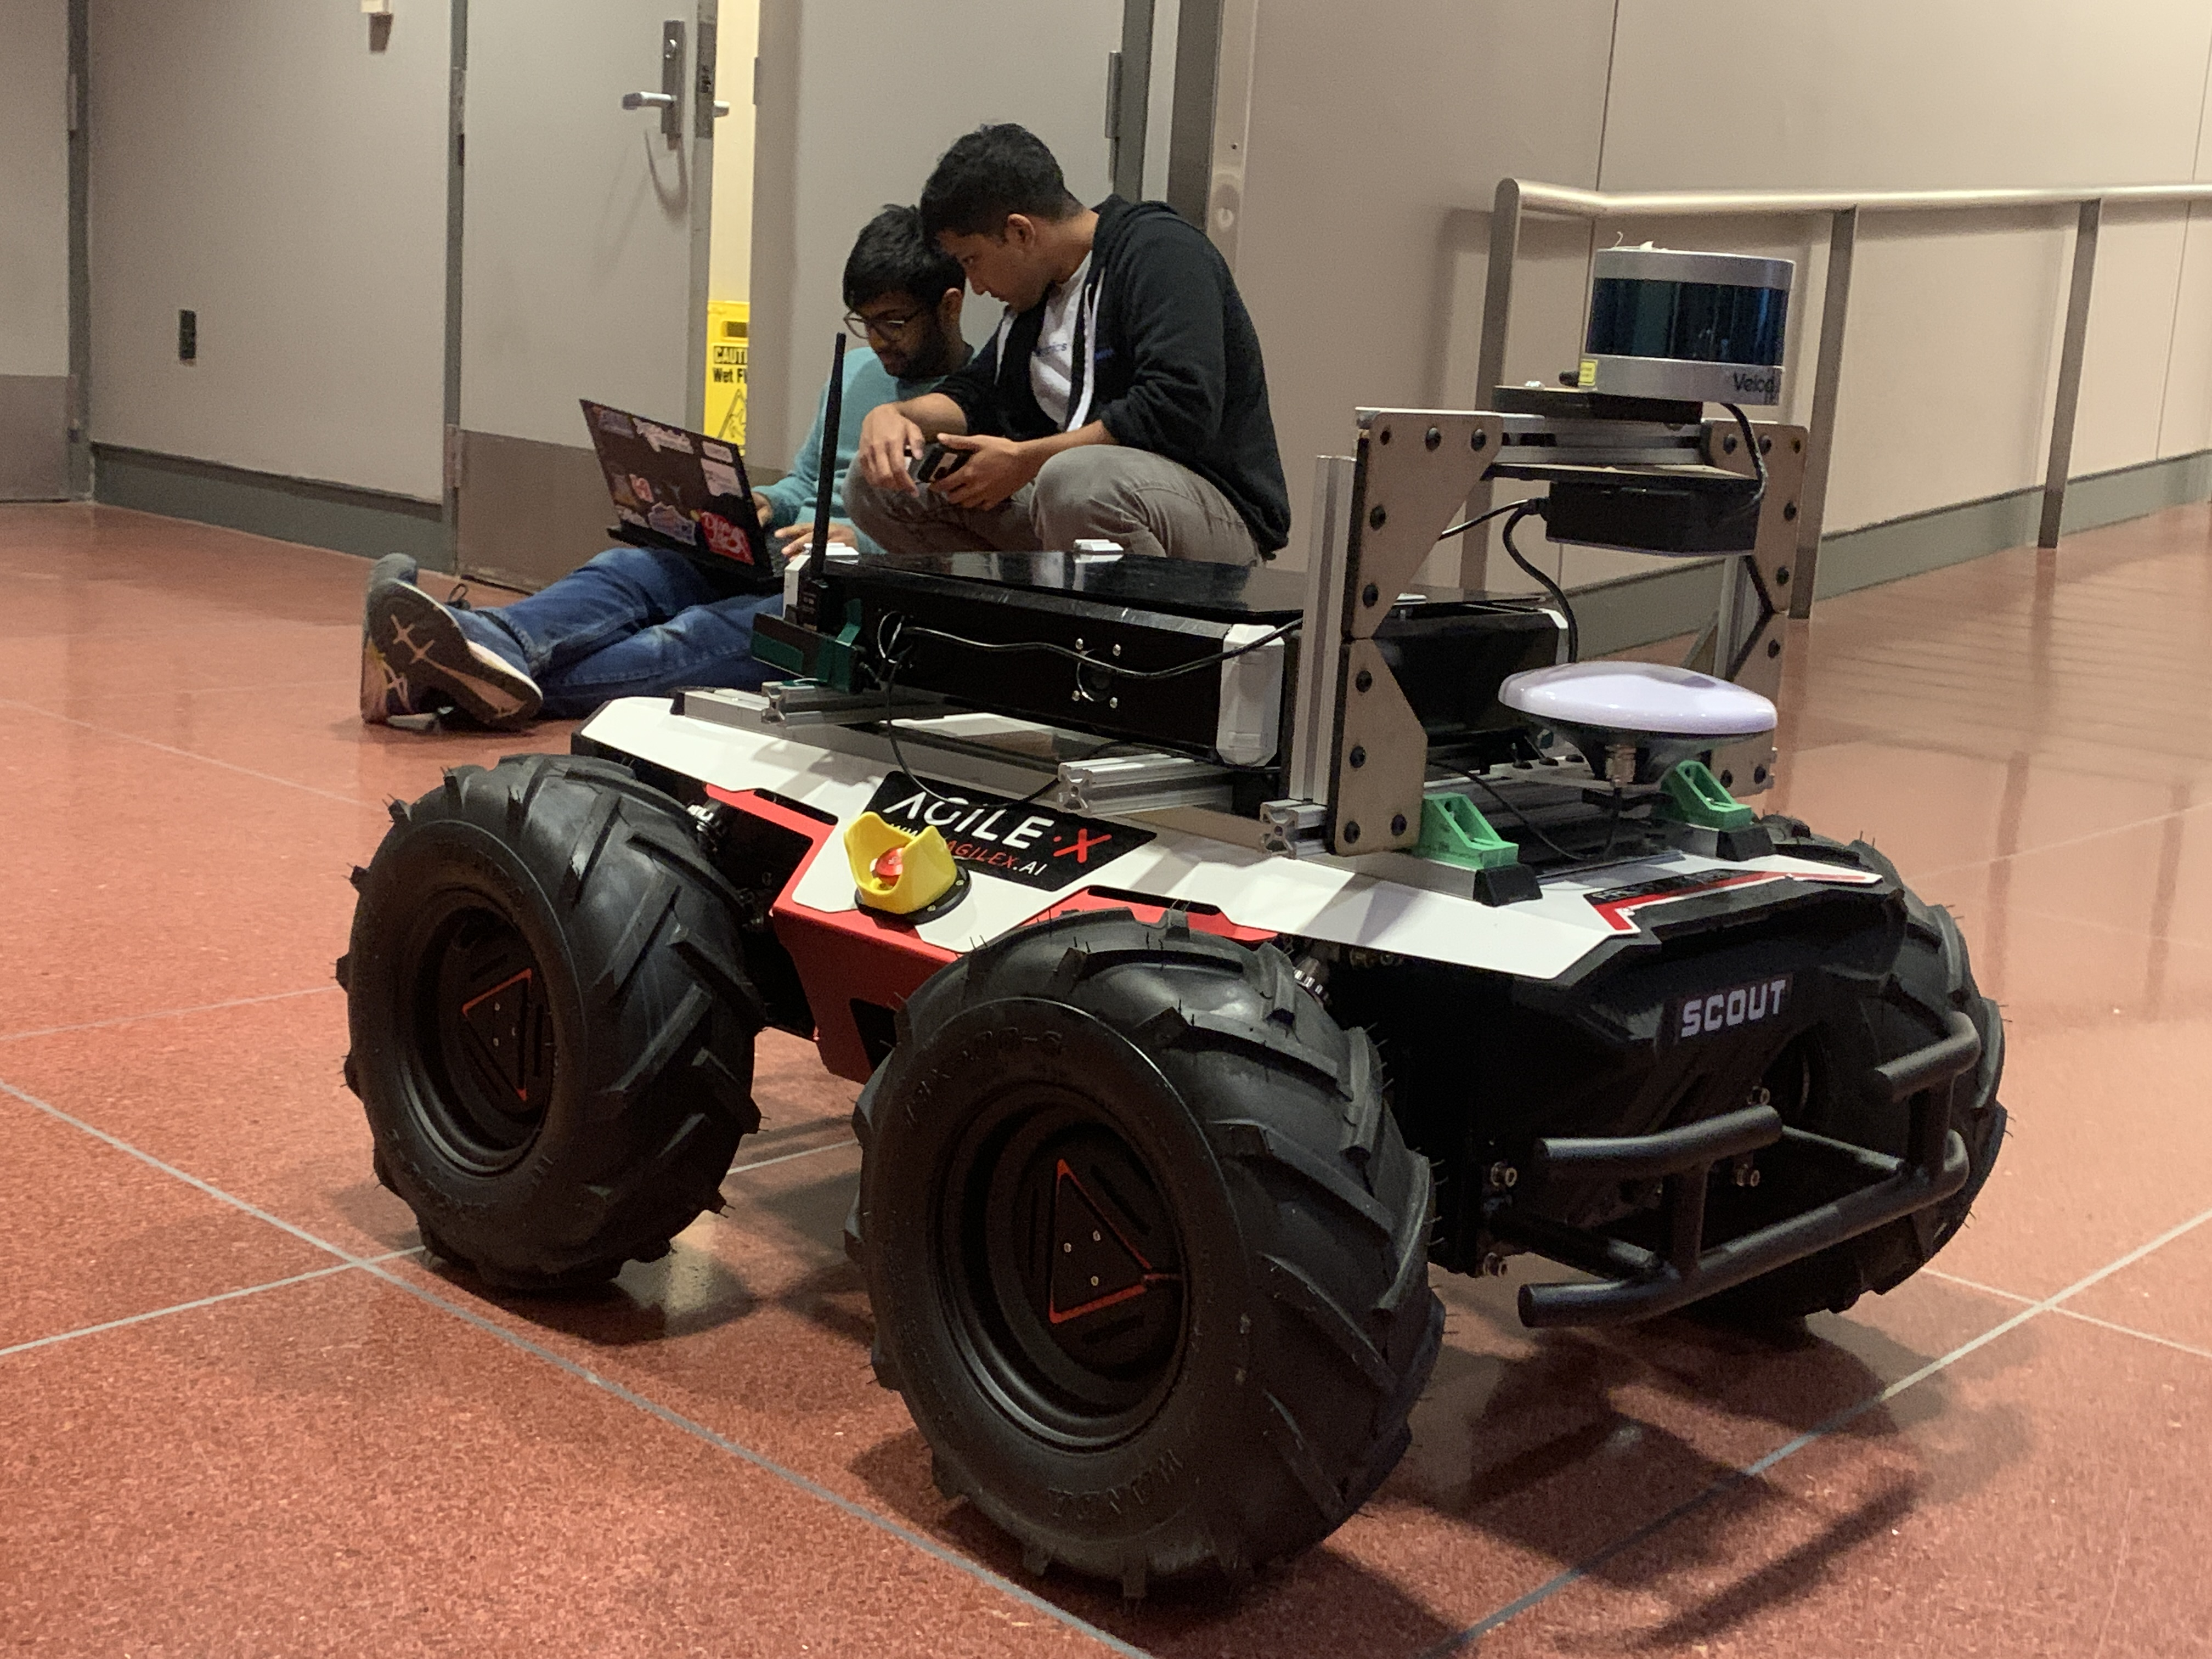
\includegraphics[width=0.48\textwidth]{images/robot_working.JPG}
  \end{center}
  \caption{AgileX Scout 2.0 with Velodyne LiDAR and GPS antenna}
    \label{fig:robot}
\end{wrapfigure}

\subsection{Hardware Setup}
We sourced a ground vehicle - AgileX Scout 2.0 - for mapping and testing from Prof. Nadia Figueroa. We also sourced a Velodyne Puck VLP-16 from PERCH for 3D ranging data. Figure \ref{fig:robot} shows the robot with the LiDAR and GPS antenna mounted on top. The robot is equipped with a Jetson Xavier NX for computation. We used ROS Melodic for interfacing with the sensors and the robot.


\subsubsection{\textbf{GPS setup}}
We bought a GPS antenna for better reception and hooked up a GPS module to the Robot. The module sends NMEA sentences over the serial port which are parsed using our own NMEA driver. The data from a GPS module is the current Latitude, Longitude, and Altitude of the robot. This data was transformed to the map frame of the robot using GPS to Cartesian conversion.
\begin{enumerate}
    \item Select reference origin by sampling real GPS data, $(lat_{ref}, lon_{ref})$
    \item Calculate Earth's radius at given latitude using ROS Hector plugin, $(R_{North}, R_{East})$
    \item $x = radians(lat - lat_{ref}) * R_{North}$
    \item $y = radians(lon - lon_{ref}) * R_{East}$
\end{enumerate}
This data is then published as a ROS topic, at 10Hz, to be used by the factor graph for sensor fusion.


\subsubsection{\textbf{Velodyne VL16 Puck Lite}}

We attempted to connect and test the LiDAR but initially faced issues interfacing with the device. After many attempts, we were able to determine that it was a hardware issue and got another LiDAR which was in working condition. We set up the drivers and tested it on our hardware and the robot.

We also got wiring and routed the power from the robot power supply to the Velodyne Puck, and connected it to the Jetson on board through ethernet. 

\subsubsection{\textbf{Assembly}}
We fabricated a mount for the LiDAR and the GPS antenna using 80-20 rods cut to size. We designed MDF brackets, which we laser cut to assemble the mount and attach it to the robot. 

The LiDAR was firmly mounted above the GPS and compute board to get an unobstructed view of the surroundings. The GPS antenna was mounted on the top of the robot to get a clear view of the sky.

\subsection{Algorithms}
This section describes the algorithms we implemented and the packages we used for mapping, localization, control, and sensor fusion.
\subsubsection{\textbf{HDL Graph SLAM and Localization}}
We utilized the HDL Graph SLAM library \cite{hdl2019} to create a 3D point cloud map of Levine Hall, Towne, and the outdoor area near it. Figure \ref{map} shows the map in RViz, the feature-rich indoor environment can be differentiated from the outdoor space. This dense point cloud is used to localize by matching current LiDAR point clouds with the map. 
\begin{wrapfigure}{R}{0.4\textwidth}
  \begin{center}
    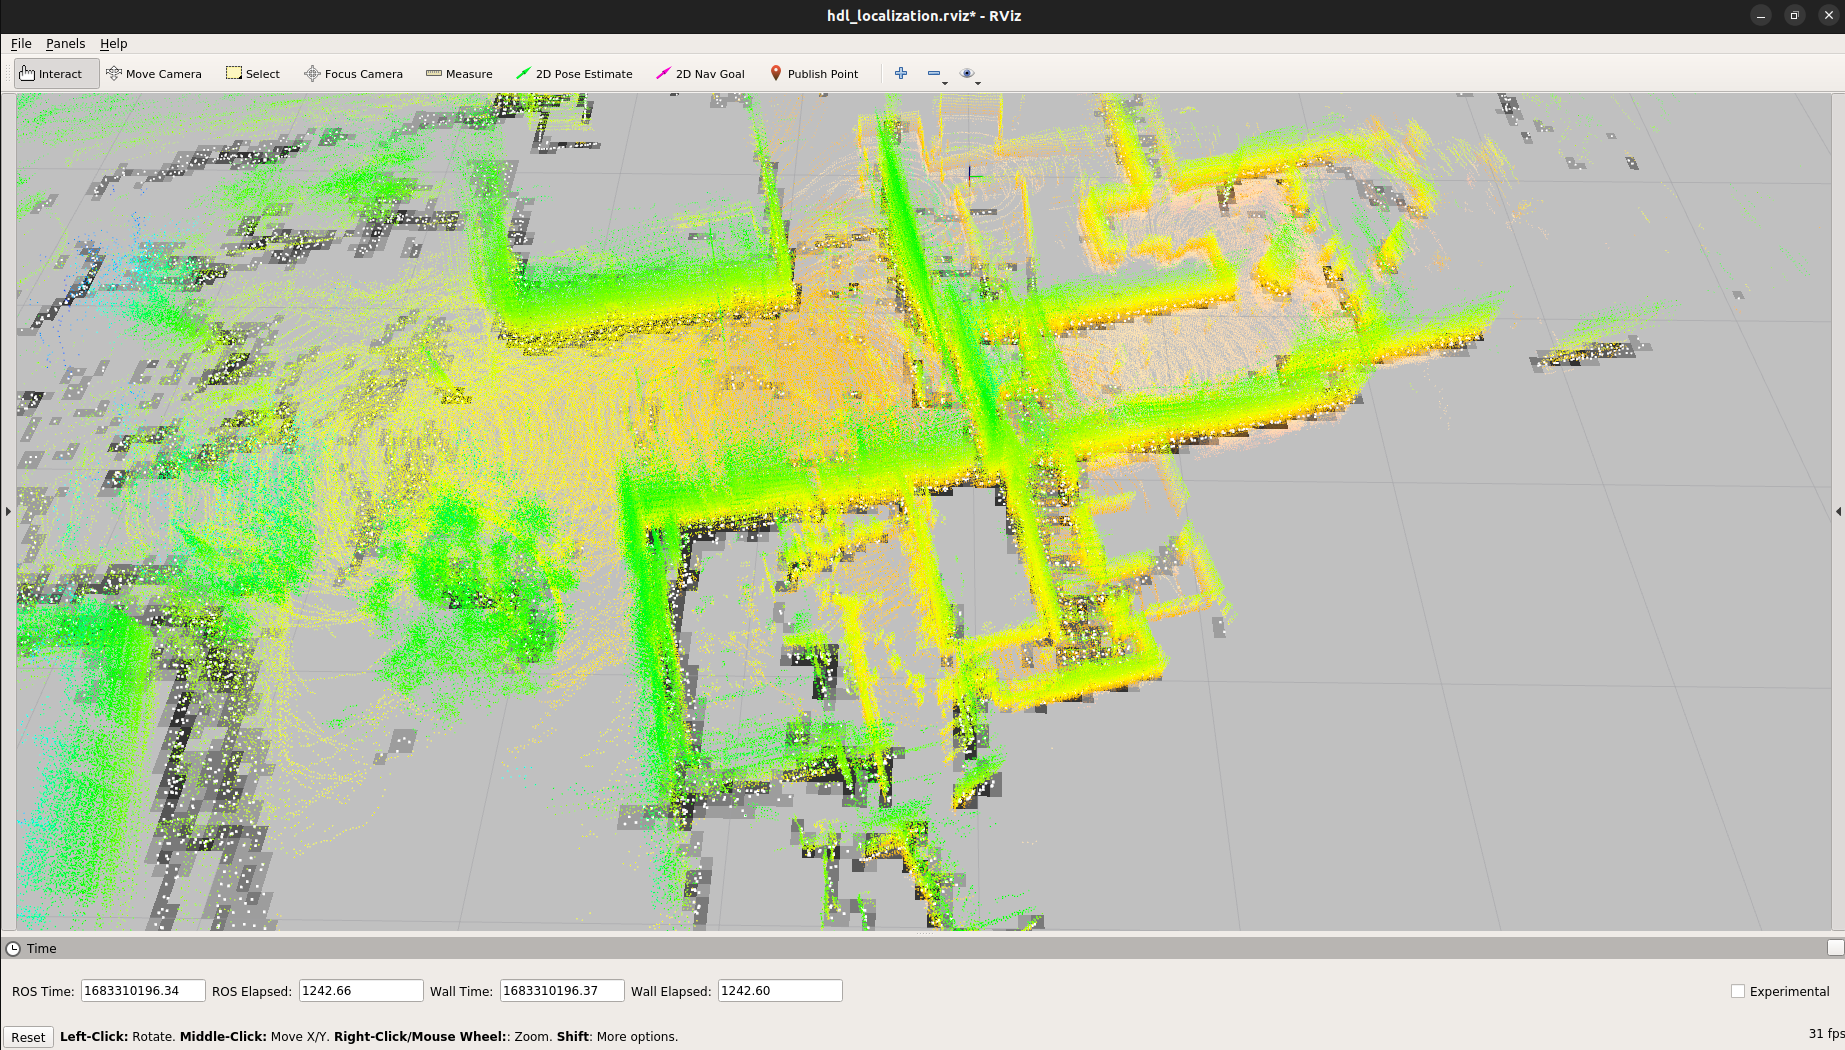
\includegraphics[width=0.5\textwidth]{images/map_with_pointcloud.png}
  \end{center}
    \caption{Map of Levine Hall, Towne and the outdoor area near it}
    \label{map}
\end{wrapfigure}


\subsubsection{\textbf{Pure Pursuit}}
In order to track a trajectory given by way-points, a simple and robust controller is the Pure Pursuit \cite{pure_pursuit_1992}. This controller tracks the projection of a point at a ‘look-ahead’ distance from the robot and corrects the turning in proportion to the curvature to get to the point. It can be modified extensively for different applications. But as this is not the primary goal of the project and as our robot is following a simple path, we have opted to go for a simple version with constant speed and look-ahead distance. We compute the curvature of the tracking point and scale it by a proportionality factor to command angular velocity, $\omega$. 
\begin{equation*}
    \omega = K_p * \frac{|y|}{L^2}
\end{equation*}
Where $L$ is the lookahead distance and $y$ is the lateral displacement of the target point in the robot frame. 
Where we use $L  = 2m$ and $Kp = 1.0$ and run the robot with constant speed $v = 0.5m/s$. Figure \ref{pure_pursuit} shows the robot following the path in the map.
\begin{figure}
     \centering
     \begin{subfigure}[b]{0.45\textwidth}
         \centering
         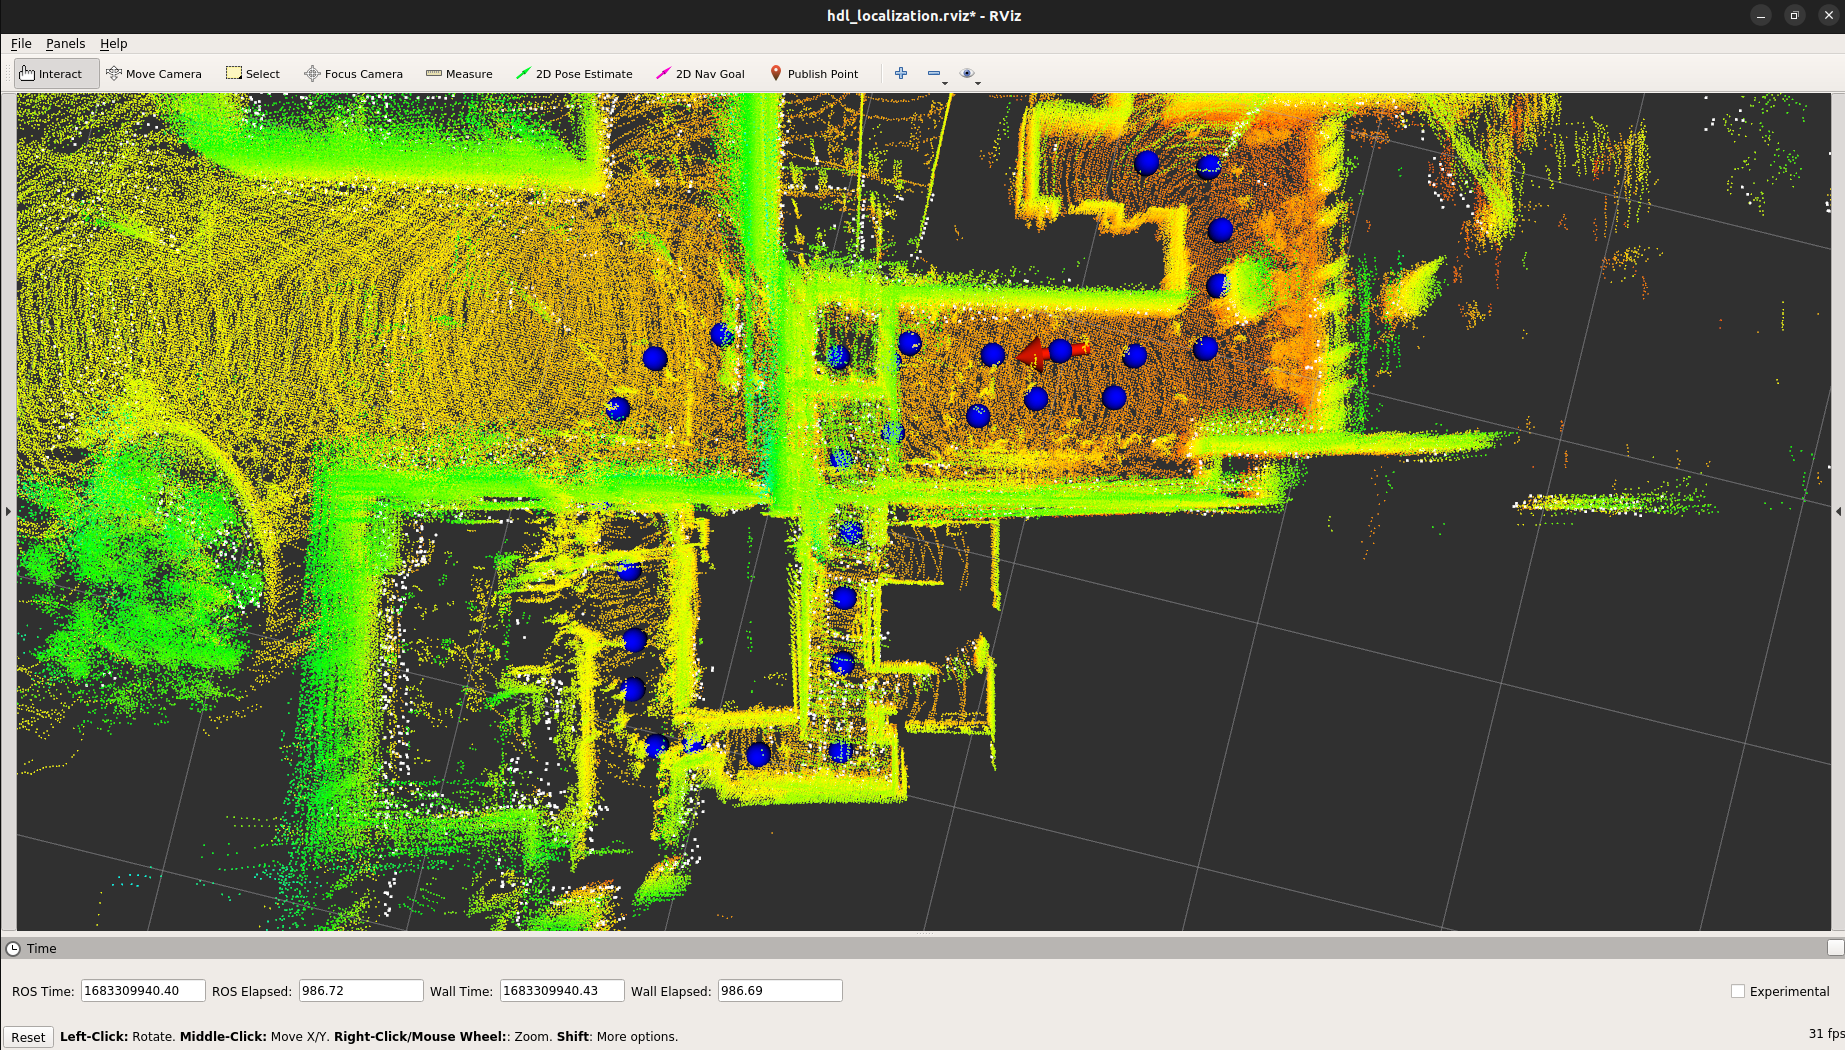
\includegraphics[width=\textwidth]{images/pure_pursuit.png}
         \caption{Pure Pursuit}
         \label{pure_pursuit}
     \end{subfigure}
     \hfill
     \begin{subfigure}[b]{0.45\textwidth}
         \centering
         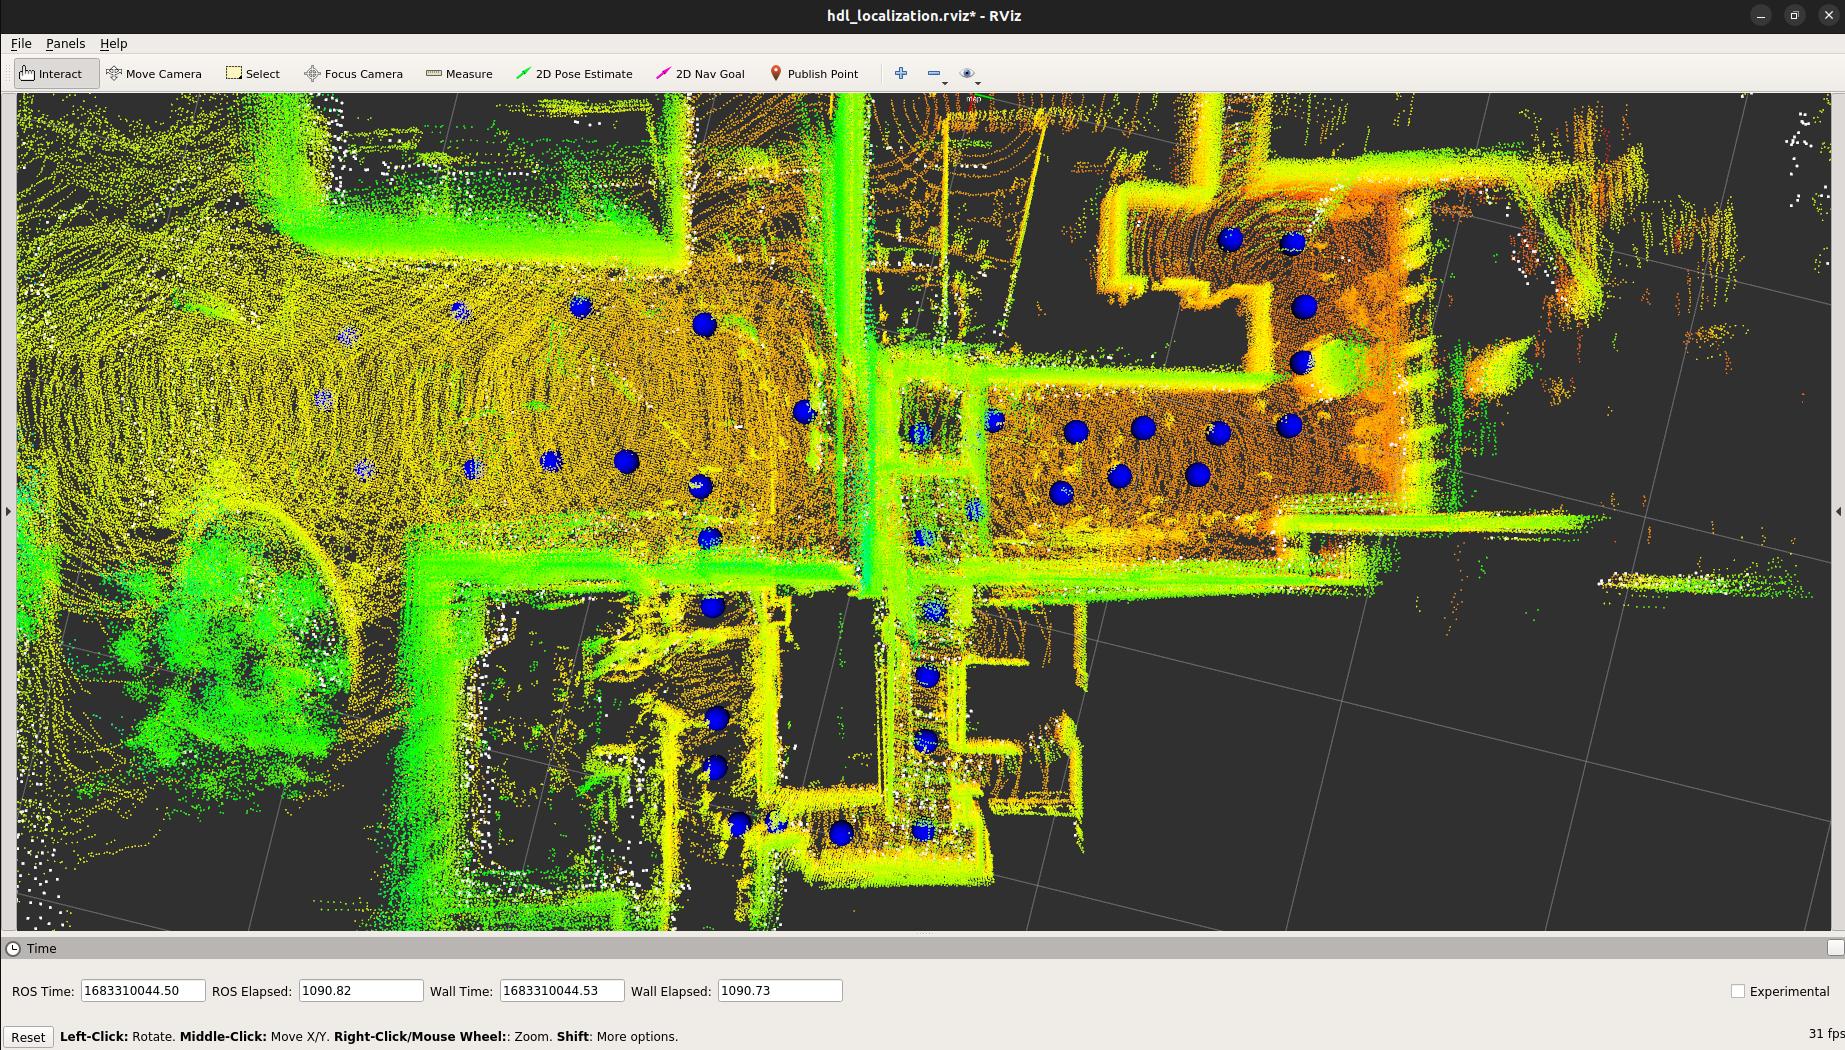
\includegraphics[width=\textwidth]{images/waypoints_big.png}
         \caption{Pure Pursuit waypoints outside the building}
         \label{pure_pursuit_outdoor}
     \end{subfigure}
        \caption{Pure Pursuit and Waypoints}
        \label{pure_pursuit_waypoints}
\end{figure}

\subsubsection{\textbf{Sensor Fusion using Factor Graphs}}
We have three different factor layouts for each of our measurements. We defined a custom \emph{Unary} factor structure to represent our location reading.

Every time we receive a measurement reading from any source, we add a new pose node to the graph.
Our odometry information is incorporated as a \emph{BetweenFactor} that connects the previous node to the new pose node. The \emph{Unary} factor corresponding to the measurement is modeled as a Gaussian factor and added to the new node. Information from multiple sensors is added as independent \emph{Unary} factors to the current node.
If multiple sensors give information then more \emph{Unary} factors are added to the current node. 

After setting initial values to the nodes in the graph, we perform inference and obtain an a posteriori estimate of the current robot state. We continue to build the graph as the robot moves to perform filtering, \ref{eqn: filtering}. All the older nodes in the factor graph get updated with the smoothing estimates, \ref{eqn: smoothing}.

\begin{equation}
    \label{eqn: filtering}
    \text{Filtering: }P(X_i | Y_0, \dots , Y_i, X_0, \dots, X_i)
\end{equation}
\begin{equation}
    \label{eqn: smoothing}
    \text{Smoothing: }P(X_k | Y_0, \dots , Y_i, X_0, \dots, X_i); k<i
\end{equation}
In order to make the robot perform both indoor and outdoor localization, we would use a noise model with small covariance for indoor localization and when we exit a building we increase the covariance of the noise model for reducing confidence in these LiDAR-based estimates. When we enter back into the building, we increase confidence. We do this by defining two-factor models for the LiDAR – indoor and outdoor. The GPS estimates are only factored into the graph when we are in the outdoor section of the map.

\section{Experimental Results}

\subsection{Pure Pursuit and Waypoints}
Waypoints are hand-selected from the map and the robot is commanded to follow them using Pure Pursuit. Figure \ref{pure_pursuit} shows the robot following the path in the map. Multiple runs of the given waypoints were performed and the robot was able to follow the path with minimal error.
To test outdoor localization using purely LiDAR, we commanded the robot to follow a path outside the building. The robot was able to follow the path with minimal error inside the building and performed poorly once it went far away from the building. Figure \ref{pure_pursuit_outdoor} shows the  waypoint trajectory outside the building.

The performance of the robot while traversing indoor and outdoor regions of the trajectory can be viewed in the following simulation capture and real footage: (\href{https://drive.google.com/file/d/1S5dACtsnclNLarxH920A84mAjVBbkHSJ/view?usp=share_link}{RViz indoors}, \href{https://drive.google.com/file/d/1_K32a5YyUOGGNr-nXjuIZ-EI5aUw_gXX/view?usp=share_link}{camera indoors})
 (\href{https://drive.google.com/file/d/1MZhdwVj8nc3G_MShZj-Z2F_11WAOJ8Xa/view?usp=share_link}{RViz outdoors}, \href{https://drive.google.com/file/d/1QDAX6c1etOxoA3TyvnGu2bQftwHt8Psq/view?usp=share_link}{camera outdoors}).

One can see the LiDAR localization's  dependecy on feature rich environments and the need to fuse GPS data when available in outdoor environments.

In our experiments, we found that due to cloud cover, rain, and surrounding buildings, GPS readings were rarely received and wildly inaccurate when they were. We were able to receive accurate GPS readings in another location far from buildings and confirm that the GPS was working properly, but it was infeasible to test there. Thus, we performed trials on the robot only using only LiDAR data.


\subsection{Localization using Fused Estimate}
In order to demonstrate the functioning of our algorithm, we used the trajectory we designed for Levine and around as ground truth and then simulated sensor data as a noisy version of this. We used realistic noise models, where the LiDAR localization indoors is accurate and suddenly fails completely outdoors. For odometry, we simulated drift which is often observed and for GPS, noisy information, is available only outside. We then used our factor graph to fuse the data and track the trajectory. 

In our factor graph, measurement factors were modeled as Gaussians with parameters given in Table \ref{tab:Noise}. These tuned values are of the same order of magnitude to those used to generate simulated sensor readings.

% Make a table for sensor-noise
\begin{table}[h]
\centering
\begin{tabular}{@{}lll@{}}
\toprule
Sensors used for localization & Noise Model & Noise Parameters \\ \midrule
LiDAR Localization Indoor & Gaussian & $\mu = 0, \sigma = 0.4$ \\
LiDAR Localization Outdoor & Gaussian & $\mu = 0, \sigma = 10.0$ \\
Odometry & Gaussian & $\mu = 0, \sigma = 1.1$ \\

GPS & Gaussian & $\mu = 0, \sigma = 2.0$ \\ \bottomrule
\end{tabular}
\caption{Noise Models for different sensors}
\label{tab:Noise}
\end{table}

The results can be seen in Figure \ref{fig:factor_graph}.
\begin{figure}
    \centering
    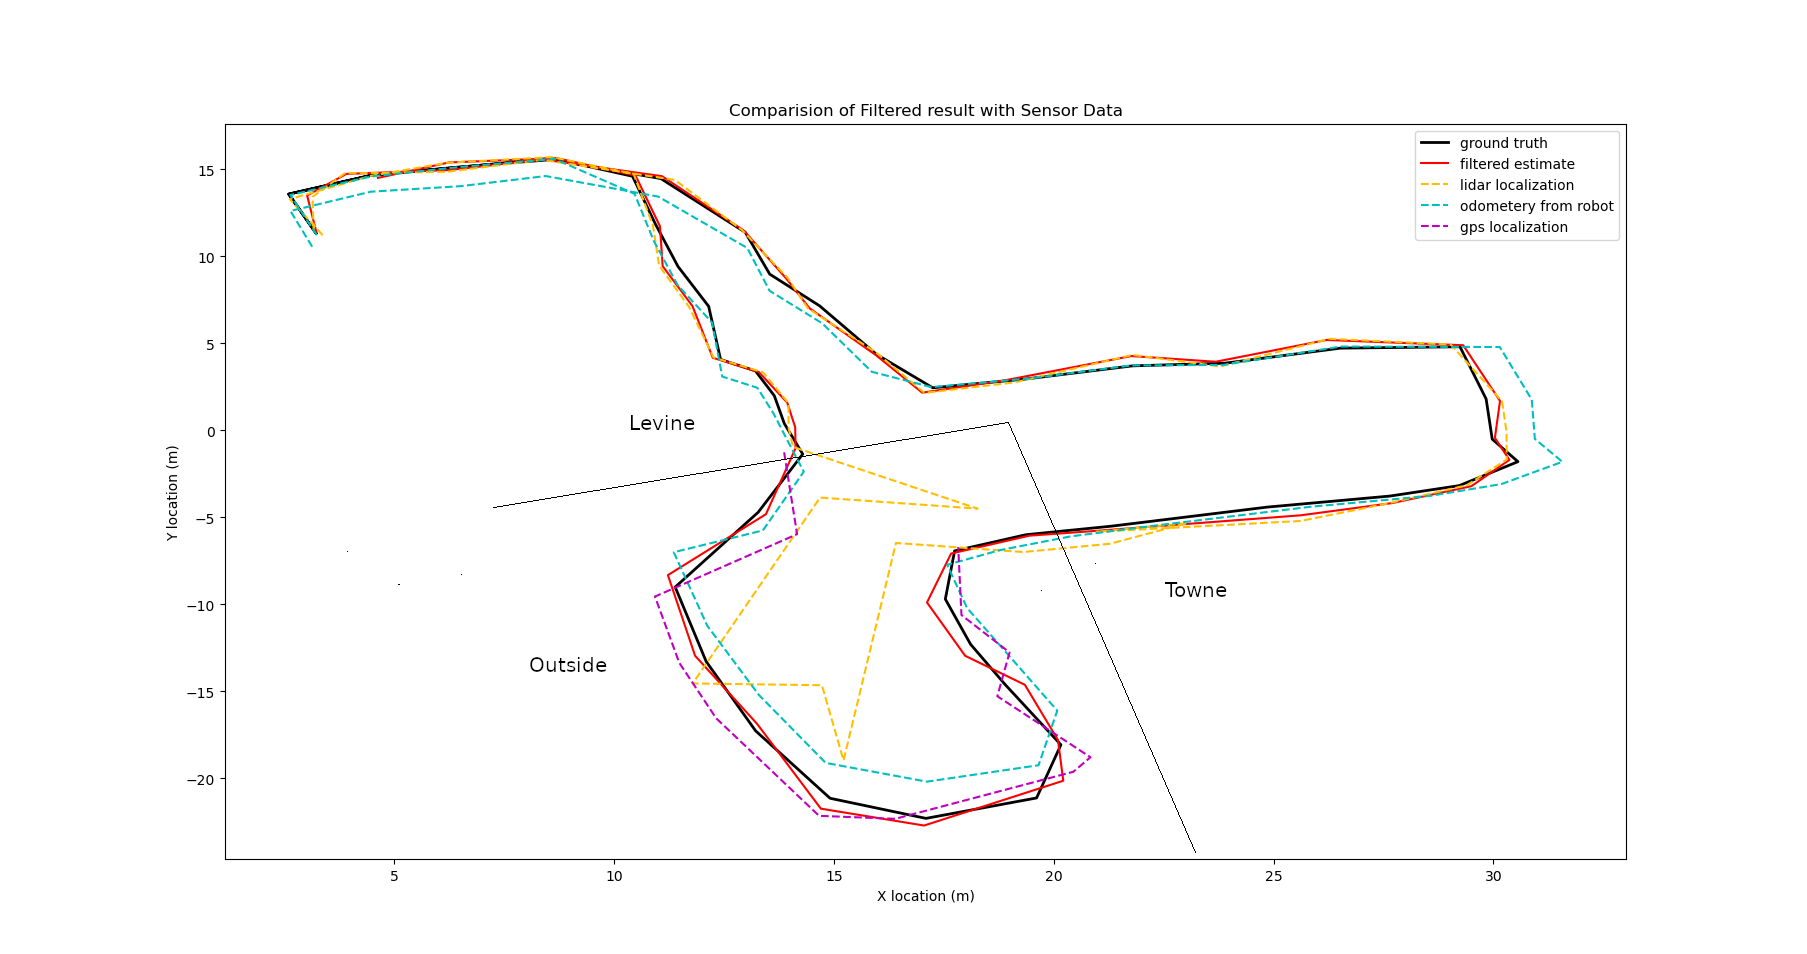
\includegraphics[scale=0.35]{images/filter_vs_sensors_2_with_outdoor.png}
    \caption{Sensor Fusion using Factor Graph}
    \label{fig:factor_graph}
\end{figure}
% \begin{figure}
%      \centering
%      \begin{subfigure}[b]{0.8\textwidth}
%          \centering
%          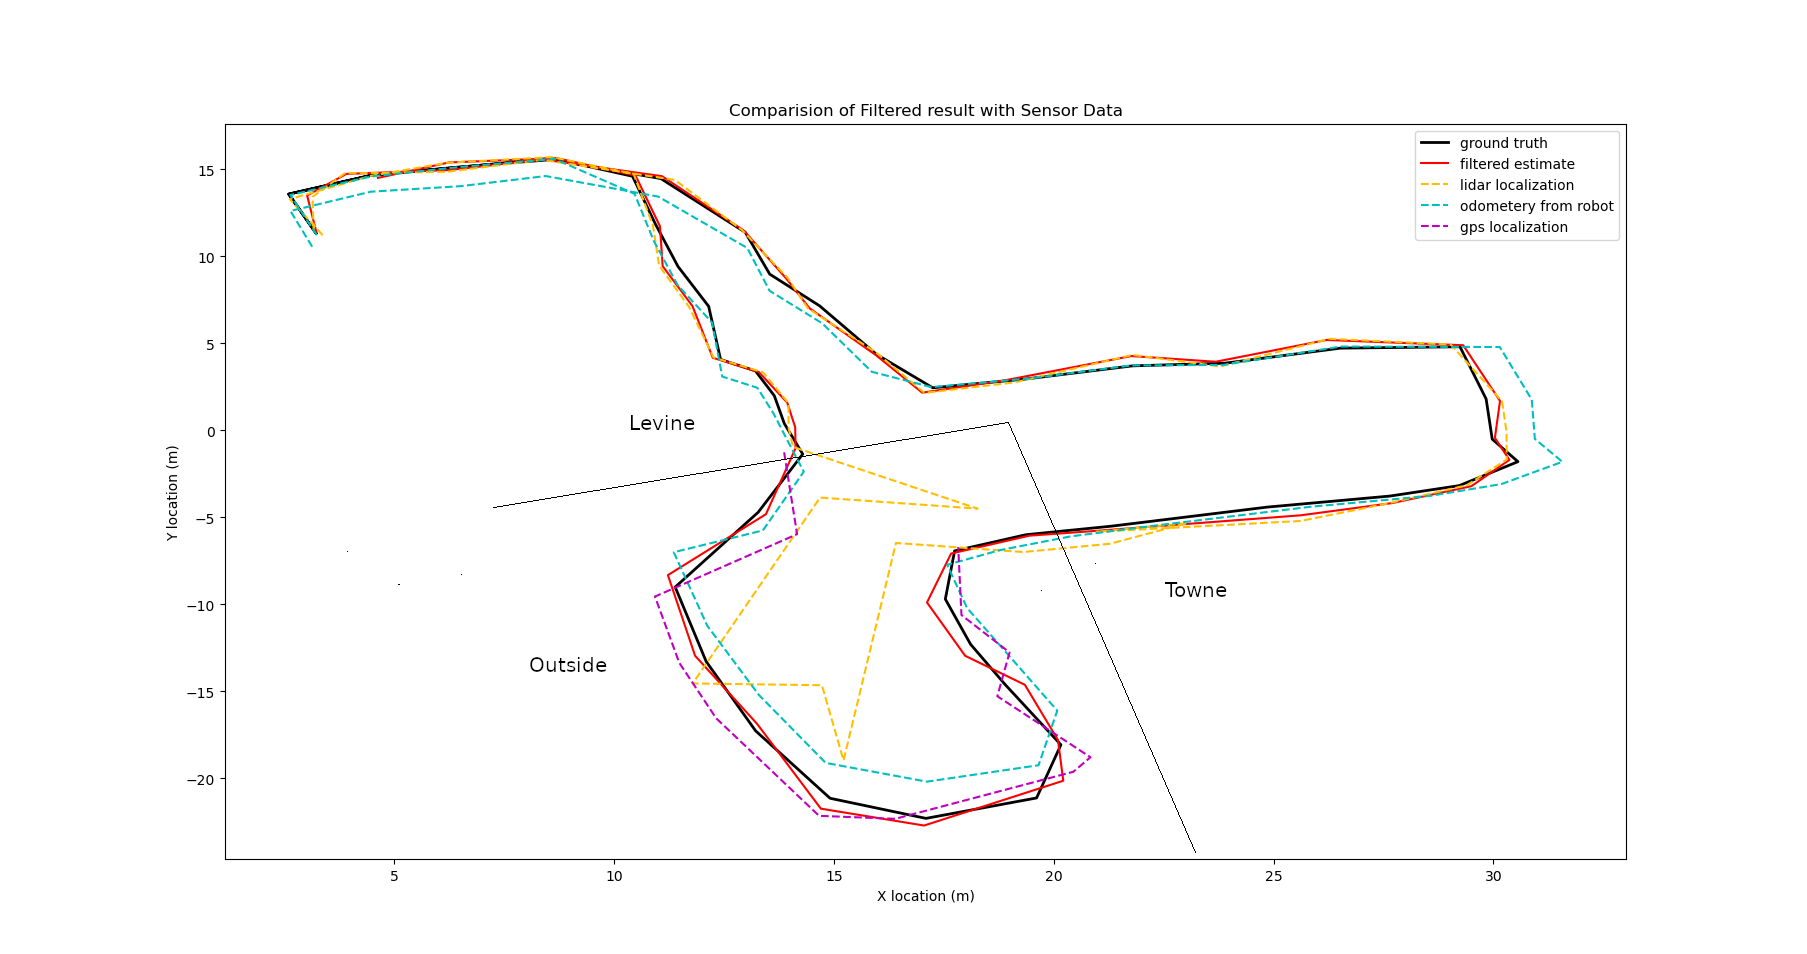
\includegraphics[width=\textwidth]{images/filter_vs_sensors_2_with_outdoor.png}
%          \caption{Pure Pursuit waypoints outside the building}
%          \label{pure_pursuit_outdoor}
%      \end{subfigure}
%         \caption{Sensor Fusion using Factor Graph}
%         \label{fig:factor_graph}
% \end{figure}

With this simulated sensor data we were able to tune our factor graph and show that we are able to track the trajectory accurately and better than just following any particular sensor. The results can be seen in the graphs above.

Note that GPS is available only outside, odometry has drift in places and LiDAR is accurate inside but noisy outside the building.

\subsection{Smoothing vs Filtering}
We wanted to explore more into the difference between smoothing and filtering. We used our factor graph to get both filtering and smoothing estimates for our trajectories and observed how they differ.

As can be seen in figure \ref{fig:smoothing_vs_filtering}, there is a difference between the trajectories. Indoors the filtering and smoothing estimates match the LiDAR as it has been modeled as a good sensor indoors and therefore newer information has less impact. 
But outdoors, where the LiDAR model is modeled to be unreliable, the trajectory between smoothing and filtering differs as no single sensor weighs in on the location. The GPS data is noisy and this impacts the filtering  output while the smoothing results follow the intended trajectory.
This was an interesting result to note which confirms the concepts taught in class.

\begin{figure}
    \centering
    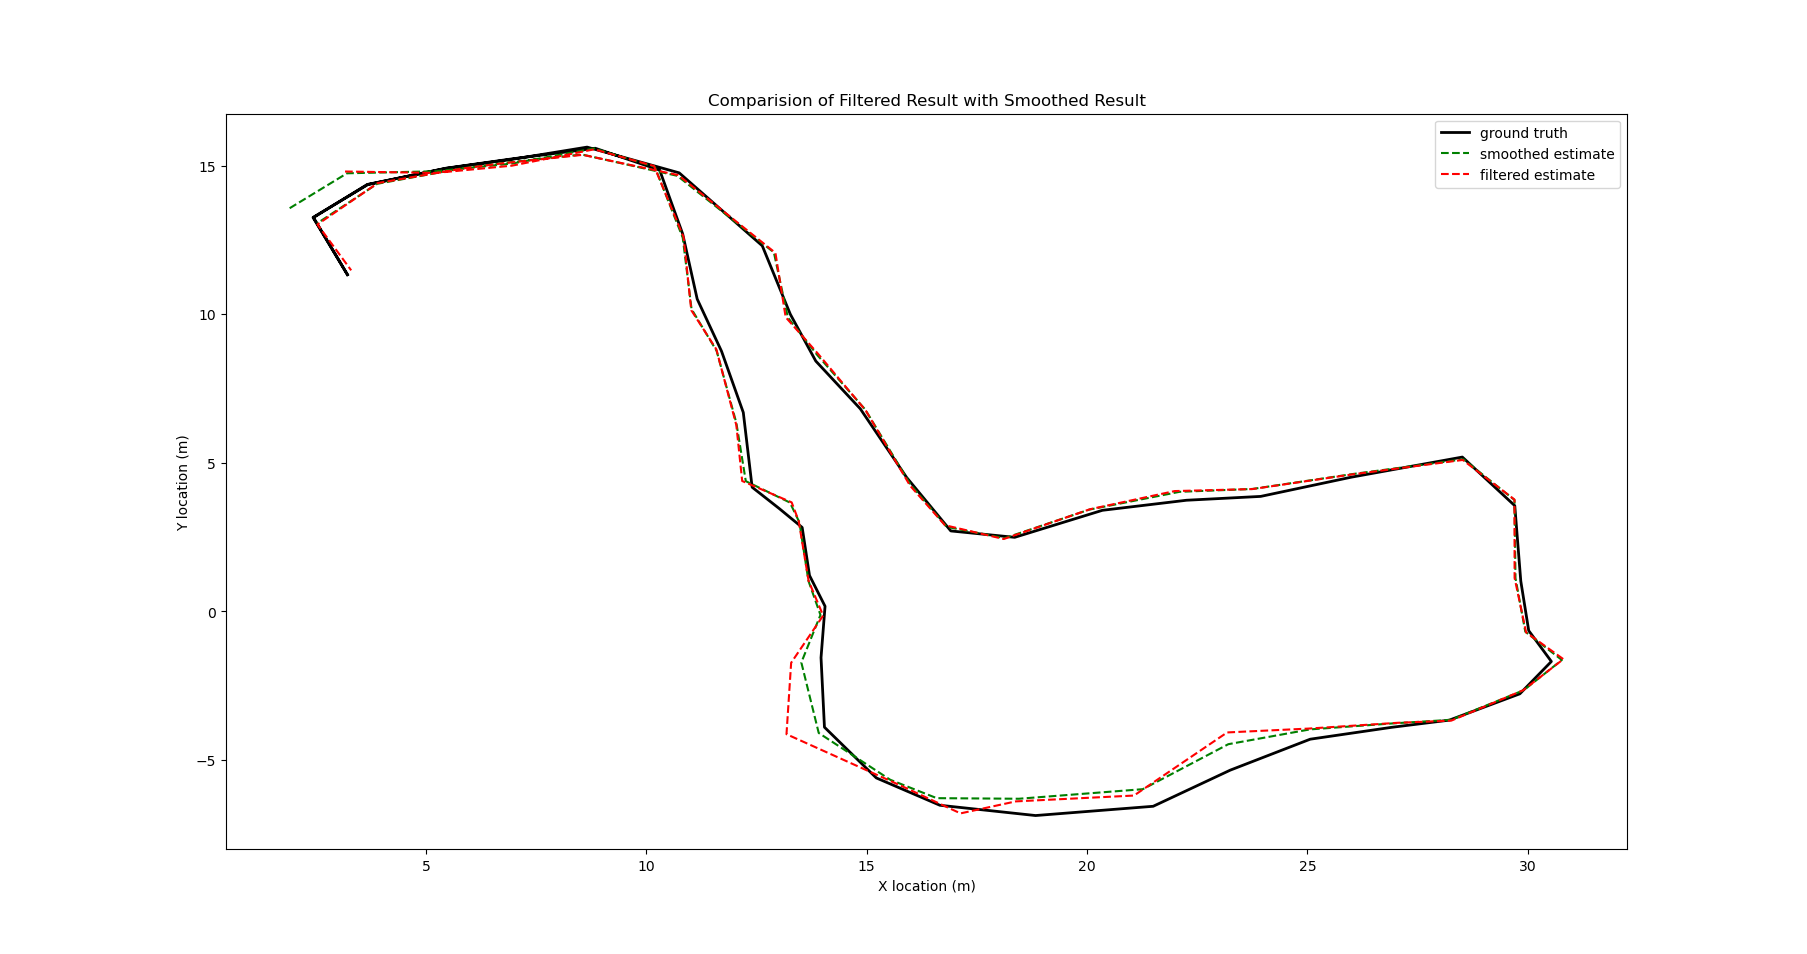
\includegraphics[scale=0.35]{images/filtered_vs_smoothed_1.png}
    \caption{Smoothing vs Filtering}
    \label{fig:smoothing_vs_filtering}
\end{figure}



\section{Discussion}
The overall goal of the project was to implement sensor fusion on the real robot and track a loop that goes from an indoor setting to outdoor and back. We were able to perform this for a smaller loop using only LiDAR localization, but the results from simulation show promise for the factor graph approach.
We chose this project as it gave us a chance to work with a real robot, implement algorithms for localization and sensor fusion and discover the challenges that come with working with real hardware. 

During setup, we faced issues with the LiDAR and GPS hardware and had to troubleshoot them. GTSAM, Docker, Linux and ROS distros all posed similar setup delays but gave us insight and valuable knowledge regarding debugging and setting up real robots for projects. We also had to learn how to use the GTSAM library and the factor graph approach to localization. 

Given more time, we would relocate our trials to an environment like Pennovation, as it has a RTK basestation, giving us a higher chance of recieving more accurate GPS data. This would permit us to test our sensor fusion algorithm in the loop with real data on the robot. However, our trouble in this respect highlights that the indoor-outdoor problem is one worth attention, as there are many environments in which localiaztion is hard to achieve even with different sensing modalities.
\section{Acknowledgements}

We would like to extend our gratitude to those who enabled our work. Thanks to Dr. Nadia Figueroa for welcoming us into the lab space and for generously providing us with the AgileX Scout 2.0 platform. Thanks to Fernando Cladera for supplying us with the Velodyne LiDAR and all the hardware and firmware troubleshooting assistance thereafter. Finally, thanks to Dr. Pratik Chaudhari for his assistance with project formulation and for providing insight regarding factor graph implementation and the GTSAM library.
% \section*{References}
\clearpage
\bibliographystyle{IEEEtran}
% Include bibliography file
\bibliography{IEEEabrv,references}

\end{document}